\begin{figure}[h]
	\centerline{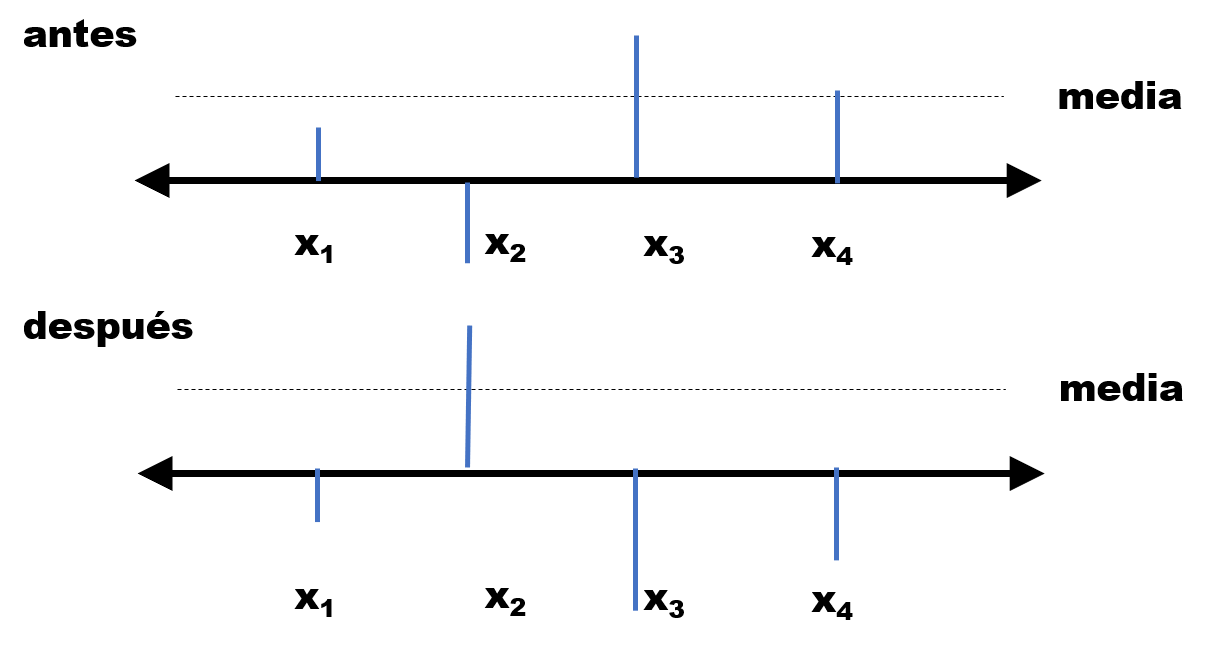
\includegraphics[scale=0.4]{figuras/inversionmedia.png}}
	\caption[Inversión sobre la media del algoritmo de Grover]{Inversión sobre la media del algoritmo de Grover. El conjunto de ${x_i}$ son las amplitudes de cada estado cuántico. La línea discontinua es la media de las amplitudes. Después de cada inversión, la amplitudes grandes se vuelven más grandes y las pequeñas más pequeñas. Fuente: elaboración propia}
	\label{fig:inversionmedia}
\end{figure}

En la Figura~\ref{fig:inversionmedia} vemos que es una figura de elaboración propia, mientras que la Figura~\ref{fig:distprob}, la fuente es un artículo cuya referencia viene indicada y el artículo es incluído en la Bibliografía.
\newline
\begin{figure}[h]
	\centerline{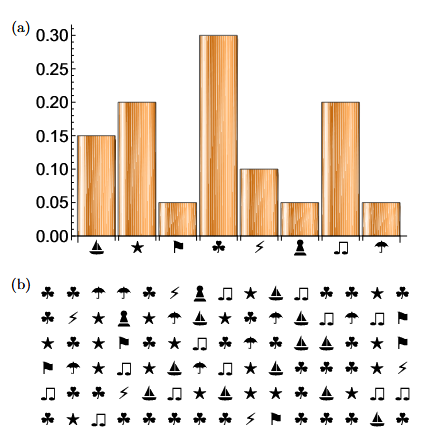
\includegraphics[scale=0.6]{figuras/distribucionprobabilidades.png}}
	\caption[Distribución de probabilidades]{a) Un ejemplo de distribución de probabilidad sobre 8 símbolos. (b) 100 muestras aleatorias de la distribución de probabilidad.
		probabilidad. El objetivo de un problema de muestreo es calcular muestras como las secuencias mostradas en (b) cuya complejidad	puede ser diferente a la complejidad de calcular la distribución de probabilidad (a). Fuente: \cite{lund2017}}
	\label{fig:distprob}
\end{figure}